\section{\emph{App}-Server}
\label{sec:appserver}
Dieser Abschnitt behandelt das Openshift Projekt \emph{App}-Server, das die gebauten Services beinhaltet. In dieses Projekt wird der freigegebene Service vom Jenkins Service bzw. der Jenkins Pipeline eingespielt. Wie für den \emph{Build}-Server, beschrieben in Abschnitt \ref{sec:buildserver-scripts}, wurden auch für den \emph{App}-Server Skripte für das Verwalten des Clusters entwickelt :
\begin{enumerate}
	\item Im \emph{Skript} \textbf{\emph{openshift-appserver.sh}} sind alle Funktionalitäten für das Verwalten des \emph{App}-Servers implementiert.
	\item Im \emph{Skript} \textbf{\emph{openshift-secrets.sh}} sind alle Funktionalitäten für das Verwalten von \emph{Secrets} implementiert. Siehe Abschnitt \ref{sec:buildserver-secrets} für eine genauere Beschreibung von \emph{Secrets}.
\end{enumerate}

\begin{figure}[H]
	\centering
	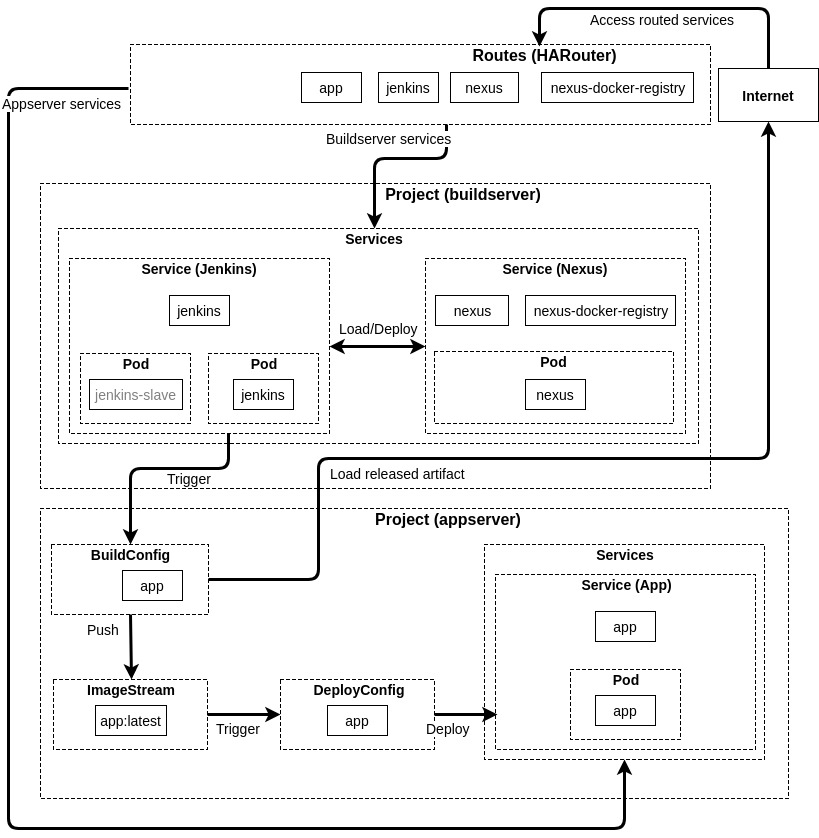
\includegraphics[scale=0.4]{logos/architecture-diagram-appserver.jpg}
	\caption{\emph{App} Server Architektur}
	\label{fig:appserver}
\end{figure}
\ \newpage

\subsection{\emph{Update}-Szenarien}
Dieser Abschnitt behandelt die \emph{Update}-Szenarien der Beispielanwendung, die in Jenkins über eine Jenkins Pipeline gebaut wird. Für diese Anwendung gibt es nur ein \emph{Update}-Szenario, nämlich wenn ein Jenkins Pipeline \emph{Build} eine neue Version freigibt, die neu eingespielt werden muss. \\

Die Jenkins Pipeline löst eine \emph{Build}-Konfiguration aus, die das neue Docker Image baut, wobei im Anschluss ein \emph{ImageChagne} Trigger ausgelöst wird, der den Service mit dem neuen Docker Image neu einspielt.
\begin{figure}[H]
	\centering
	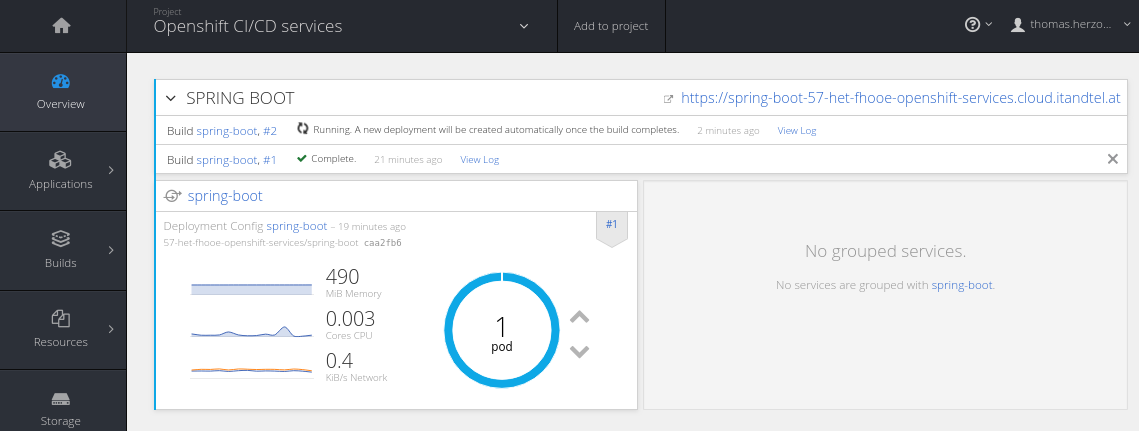
\includegraphics[scale=0.55]{image/service-app-redeploy.png}
	\caption{Ausrollen einer neuen Version des Service}
	\label{fig:appserver}
\end{figure}
\begin{figure}[H]
	\centering
	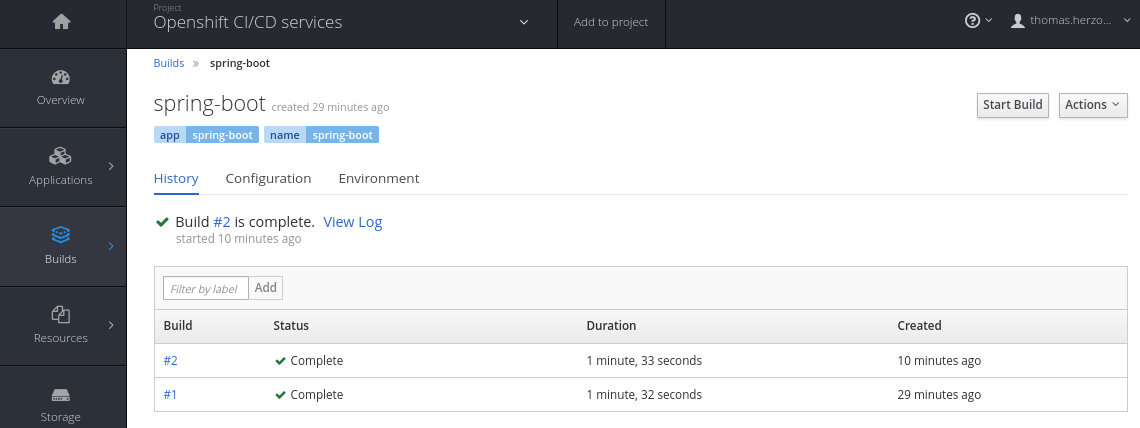
\includegraphics[scale=0.55]{image/service-app-builds.png}
	\caption{Erfolgte \emph{Builds} im \emph{App}-Server}
	\label{fig:appserver}
\end{figure}

